\subsection{Il protocollo}

\begin{frame}{Signal Protocol}
    \framesubtitle{Il protocollo}
    Il protocollo Signal fornisce crittografia end-to-end a sistemi di messaggistica istantanea e di chiamate vocali, combinando l'algoritmo \textbf{``Double Ratchet''}, pre-chiavi e un triplo handshake Elliptic-curve Diffie–Hellman (3-DH). 
\end{frame}

\begin{frame}{Signal Protocol}
    \framesubtitle{Il protocollo}
    Le specifiche di riferimento sono infatti: \cite{signal}
    \begin{itemize}
        \item \textbf{X3DH}: protocollo di negoziazione delle chiavi Extended Triple Diffie-Hellman.\pause
        \item \textbf{Double Ratchet}: algoritmo utilizzato da due parti per lo scambio di messaggi basato su una chiave segreta condivisa. \pause
        \item \textbf{Sesame}: gestisce le sessioni crittografate in ambiente asincrono e multi-device.
    \end{itemize}
    
    \note{
        \begin{itemize}
            \item Double Ratchet: le due parti derivano nuove chiavi per ogni messaggio in modo tale che chiavi usate in precedenza non possano essere ricavate dalle chiavi successive (grazie alla non invertibilità della funzione ratchet) 
            \item X3DH: stabilisce una chiave segreta condivisa da due parti che si autenticano a vicenda basandosi su chiavi pubbliche. X3DH fornisce \textit{forward secrecy} e \textit{cryptographic deniability}
        \end{itemize}   
       
        \textit{Cryptographic deniability}: l'esistenza di un file cifrato o di un messaggio è rinnegabile, nel senso che un altro utente non può dimostrare che i dati in \textit{plaintext} esistono. Gli utenti possono negare che dei dati siano cifrati o anche negare di essere in grado di decifrarli, indipendentemente dal fatto che ciò sia vero o meno.
    }
\end{frame}

\begin{frame}{Signal Protocol}
    \framesubtitle{Il protocollo: fasi di funzionamento \cite{VanDam}}
    \begin{itemize}
        \item KEY REGISTRATION: invio di numerose chiavi pubbliche al server per consentire di iniziare una conversazione mentre l'altro utente non è online\pause
        \item KEY AGREEMENT: Alice riceve le chiavi pubbliche di Bob dal server e le usa, insieme alle proprie chiavi private, per generare una chiave segreta condivisa. Invia a Bob un messaggio criptato con questa chiave. Bob, ricevutolo, recupera le chiavi pubbliche di Alice dal server e calcola la stessa chiave segreta condivisa. La negoziazione delle chiavi avviene tramite X3DH\pause
        \item CONVERSATION: Alice e Bob possiedono la chiave segreta condivisa e possono conversare.
                            \begin{itemize}
                                \item DH ratchet phase
                                \item Symmetric ratchet phase                                
                            \end{itemize}
    \end{itemize}

    \note{
        \begin{itemize}
            \item KEY REGISTRATION: se Alice vuole iniziare una conversazione con Bob può chiedere al server le sue chiavi pubbliche
            \item KEY AGREEMENT
            \item CONVERSATION 
        \end{itemize}

        N.B. Symmetric ratchet phase e DH ratchet phase verranno meglio analizzati più avanti nel parlare dell'algoritmo Double Ratchet.  
    }
\end{frame}

\begin{frame}{Signal Protocol}
    \framesubtitle{Il protocollo: fasi di funzionamento}
    \textbf{Symmetric ratchet phase}\newline

    Derivazione di una nuova chiave dalla chiave segreta condivisa.\newline\pause
    Se Alice invia più messaggi a Bob senza ricevere risposta ogni messaggio sarà criptato con una nuova chiave calcolata in funzione della precedente.\newline\pause
    In questo modo solo Alice e Bob possono calcolarla (escludendo casi in cui la chiave sia compromessa)
    
\end{frame}

\begin{frame}{Signal Protocol}
    \framesubtitle{Il protocollo: fasi di funzionamento}
    \textbf{Diffie–Hellman ratchet phase}\newline

    Generazione di una nuova chiave segreta condivisa.\newline\pause
    Se Bob invia un nuovo messaggio ad Alice genera una nuova coppia di chiavi effimere. Bob usa queste chiavi per calcolarne una nuova condivisa, inviando poi la propria chiave effimera ad Alice per farle calcolare la chiave condivisa.\newline\pause
    La chiave così calcolata verrà usata in una nuova \textit{symmetric ratchet phase} per generare nuove chiavi per i messaggi.

\end{frame}

\begin{frame}{Signal Protocol}
    \framesubtitle{Il protocollo: X3DH}
    X3DH è stato sviluppato da OWS per supportare lo scambio asincrono delle chiavi. \cite{X3DH}\pause\newline
    Definizioni:
    \begin{itemize}
        \item Identity key: chiave pubblica\pause
        \item Ephemereal key: chiave utilizzabile una sola volta \pause
        \item Pre-keys: chiavi condivise col server prima dell'attivazione del protocollo\pause
        \item One-time pre-keys: insiemi di pre-keys condivisi col server prima dell'attivazione del protocollo. Il server condivide una chiave ogni volta che un utente vuole iniziare una conversazione e ne richiede un nuovo insieme quando stanno per finire\pause
        \item Signed pre-key: pre-key firmata con l'esponente dell'Identity key
    \end{itemize}

    \note{
        STANDARD DIFFIE-HELLMAN: Alice e Bob generano ognuno una chiave pubblica \textit{pk} basata su un generatore comune \textit{g} modulo \textit{m} e le proprie chiavi private (\textit{secret keys}) \textit{sk}. \\Dopodiché scambiano le chiavi pubbliche attraverso un canale (potenzialmente non sicuro) e da esse possono derivare una chiave segreta condivisa \textit{ssk}.
        \cite{diffiehellman}, \cite{diffiehellman2}
    }
\end{frame}

\begin{frame}{Signal Protocol}
    \framesubtitle{Il protocollo: X3DH}

    \begin{figure}
        \centering
        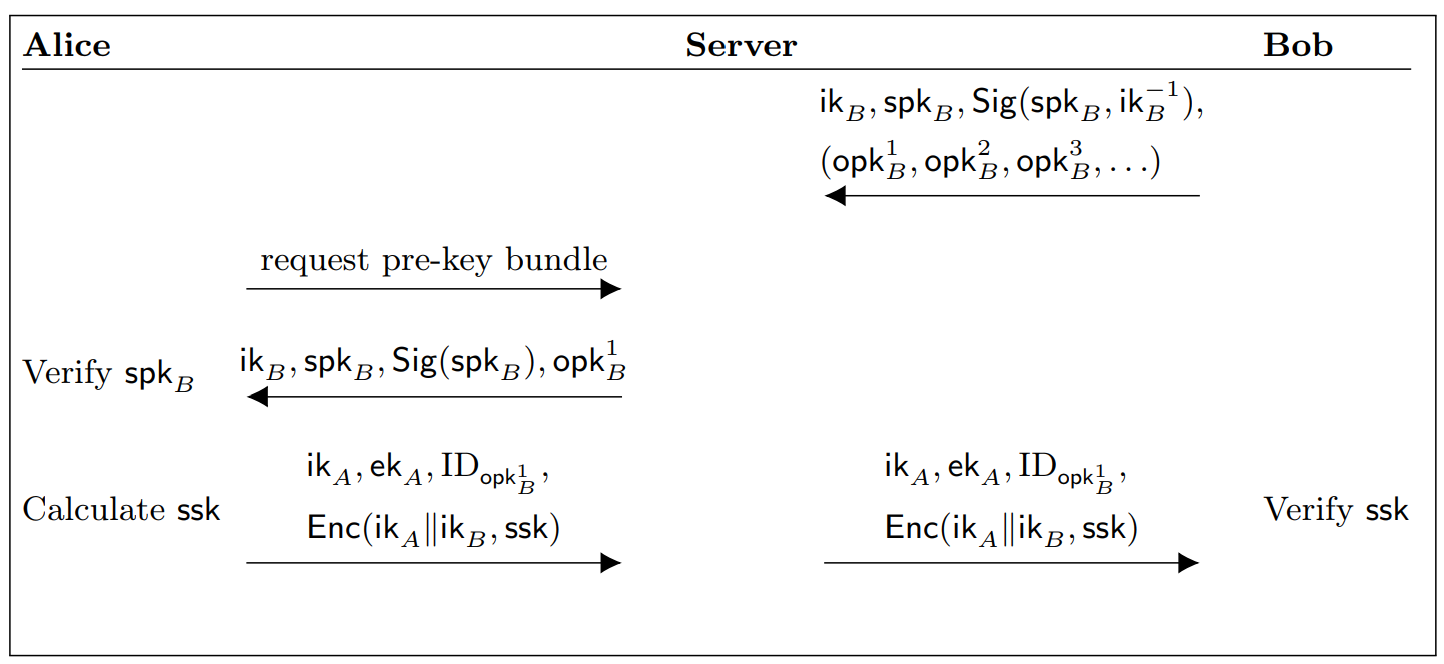
\includegraphics[width=.8\textwidth]{X3DH.png}
        \caption{Funzionamento di X3DH semplificato}
    \end{figure}

    \cite{VanDam}
\end{frame}

\begin{frame}{Signal Protocol}
    \framesubtitle{Il protocollo: Double Ratchet}

    Algoritmo utilizzato per il proseguimento della conversazione, dopo averla inizializzata tramite X3DH.\newline\pause
    \cite{doubleratchet}, \cite{VanDam} \newline   
    A differenza di X3DH usa una catena KDF, come mostrato in figura \ref{tag: KDF chain}.

    \begin{figure}
        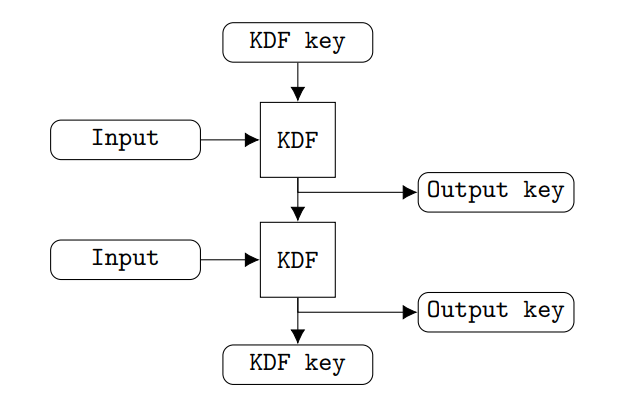
\includegraphics[width=.5\textwidth]{KDF chain.png}
        \caption{Catena KDF}
        \label{tag: KDF chain}
    \end{figure}

    \note{
        La catena KDF usa l'output di una KDF come input per un'altra applicazione della KDF.\newline
        Ogni \textit{output key} può essere utilizzata per cifrare un messaggio.\newline
        Tale catena garantisce:
        \begin{itemize}
            \item Resilienza: l'output appare randomico
            \item Forward secrecy: garantita dalla non-invertibilità della KDF
            \item Future secrecy: garantita se l'input della KDF \(i+1\) non è il solo output della KDF \(i\). Per garantire ciò è necessario usare un \textbf{DH ratchet}
        \end{itemize}

    }
\end{frame}

\begin{frame}{Signal Protocol}
    \framesubtitle{Il protocollo: Double Ratchet}
    Combinando una catena KDF con un DH ratchet otteniamo un algoritmo Double ratchet che garantisce sia \textit{forward secrecy} che \textit{future secrecy}. \newline\pause
    DH ratchet infatti modifica gli input delle KDF in modo tale che, se anche una chiave venisse compromessa, si sia in grado di ristabilire la segretezza dall'applicazione successiva di una KDF.\newline
\end{frame}

\begin{frame}{Signal Protocol}
    \framesubtitle{Il protocollo: Double Ratchet}
    Sia Alice che Bob hanno tre catene KDF da utilizzare:
    \begin{itemize}
        \item DH ratchet
        \item Sending ratchet
        \item Receiving ratchet
    \end{itemize}\pause
    Ogni volta che Alice vuole inviare un messaggio a Bob aggiornerà la catena \textit{sending ratchet} producendo una nuova chiave di output e invierà a Bob il proprio messaggio cifrato con essa.
\end{frame}

\begin{frame}{Signal Protocol}
    \framesubtitle{Il protocollo: Double Ratchet}
    La catena di invio di Alice deve essere sincronizzata con quella di ricezione di Bob e viceversa e devono iniziare nella stessa posizione (caratteristica garantita da X3DH applicato prima del Double ratchet).\newline\pause
    In queste condizioni tuttavia non è ancora garantita la \textit{future secrecy}
\end{frame}

\begin{frame}{Signal Protocol}
    \framesubtitle{Il protocollo: Double Ratchet}
    Per garantire \textit{future secrecy} Bob invierà come parte di uno dei suoi messaggi una nuova chiave pubblica Diffie-Hellman.\pause\newline
    Alice userà questa chiave per far avanzare la catena DH-ratchet, imponendo così il reset delle catene di ricezione e invio. In parallelo anche la catena DH-ratchet di Bob verrà aggiornata.\newline\pause
    Un comportamento analogo verrà applicato da Bob sulle proprie catene.\newline\pause
    Questo scambio di chiavi DH può avvenire ogniqualvolta necessario ma normalmente avviene a ogni messaggio scambiato.
    \cite{doubleratchetVid}

    \note{
        Questo sistema di catene garantisce dunque:
        \begin{itemize}
            \item Forward security: grazie alle catene di invio e ricezione, caratterizzate da funzioni non invertibili, non è possibile retrocedere ai messaggi inviati in precedenza
            \item Future secrecy: grazie alla catena DH-ratchet se anche si riesce a intercettare un messaggio e decrittarlo si resettano le catene di invio e ricezione, rendendo impossibile generare in anticipo le chiavi che verranno utilizzate in futuro
            \item Funzionamento asincrono: se Alice invia dieci messaggi a Bob e lui non risponde man mano, egli comunque sarà in grado di ricostruire la sequenza di chiavi utilizzata da Alice e dunque leggere i messaggi
            \item In ogni messaggio viene indicato il numero di messaggi già inviati sulla stessa catena quindi se un messaggio va perso si può o aspettarne l'arrivo o far avanzare la catena di tante posizioni quanti messaggi sono andati persi.
        \end{itemize}

        N.B. Le chiavi vengono eliminate non appena utilizzate per decifrare un messaggio, se delle chiavi non vengono utilizzate vengono conservate finché non arriverà il messaggio corrispondente.
    }
\end{frame}

\begin{frame}{Signal Protocol}
    \framesubtitle{Il protocollo: Double Ratchet}

    \begin{figure}
        \centering
        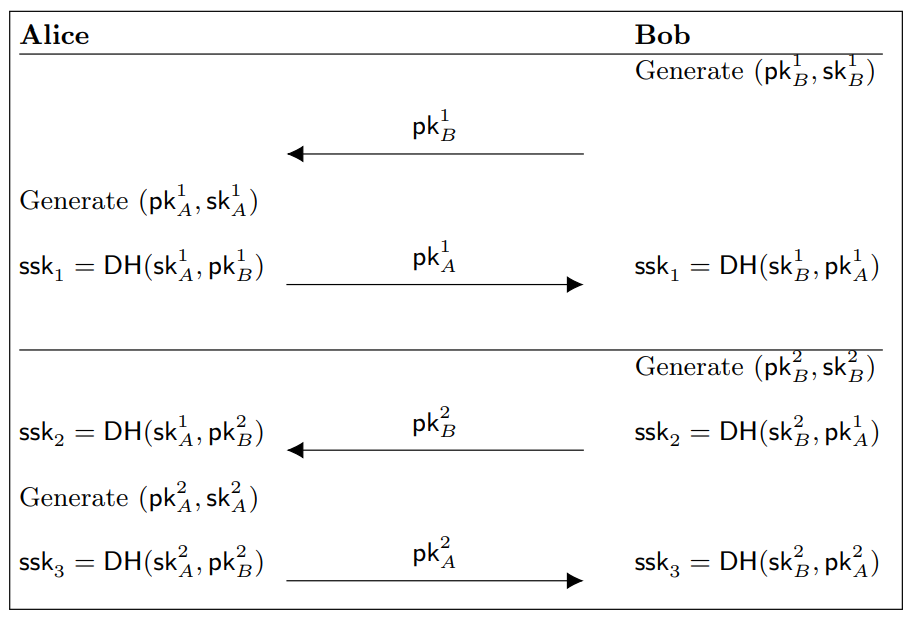
\includegraphics[width=.6\textwidth]{dh ratchet.png}
        \caption{DH ratchet}
        \label{tag: DH ratchet}
    \end{figure}

\end{frame}
\begin{frame}{Signal Protocol}
    \framesubtitle{Il protocollo: Sesame}

    L'algoritmo \textbf{Sesame} gestisce la creazione, eliminazione e utilizzo delle sessioni di comunicazione.\newline\pause
    Ogni dispositivo degli utenti deve tenere traccia di una sessione \textit{attiva} per ogni altro dispositivo con cui sta comunicando e utilizzare quella sessione quando comunica con esso.
    Quando si riceve un messaggio su una sessione \textit{inattiva}, essa diventa \textit{attiva}.\pause\newline
    In questo modo ogni dispositivo utilizza una sola sessione per ogni altro dispositivo remoto con cui comunica. 
    \cite{sesame}

    \note{
        Problemi che si possono generare:
        \begin{itemize}
            \item Alice e Bob possono avere ognuno più dispositivi quindi l'invio di un messaggio da parte di Alice richiede di inviarne una copia a tutti i dispositivi di Bob e a tutti i dispositivi di Alice.
            \item Alice e Bob possono aggiungere o rimuovere dispositivi, iniziando o terminando delle sessioni.
            \item Alice e Bob possono iniziare una nuova sessione allo stesso tempo. Per il funzionamento del Double Ratchet Alice e Bob devono usare la stessa sessione, quindi devono concordare su quella da utilizzare.
            \item Alice può resettare lo stato della sessione sul suo dispositivo, richiedendo a Bob di concordare nuovamente sulla sessione da utilizzare.
        \end{itemize}
    }
\end{frame}

\begin{frame}{Signal Protocol}
    \framesubtitle{Il protocollo: Sesame}
    Sesame è stato progettato per l'uso attraverso sessioni Double Ratchet create attraverso scambio di chiavi X3DH.

    \begin{itemize}
        \item I dispositivi comunicano al server le proprie \textit{one-time pre-keys}, \textit{signed pre-keys} e \textit{identity public key}.\pause
        \item Il dispositivo mittente recupera dal server la \textit{identity public key} del dispositivo destinatario, \textit{signed pre-keys} e una \textit{one-time pre-key} se disponibile.\pause
        \item X3DH usa queste chiavi per creare sia una chiave segreta che apre una sessione Double Ratchet sia un messaggio iniziale X3DH.
    \end{itemize}    

\end{frame}

\begin{frame}{Signal Protocol}
    \framesubtitle{Il protocollo: Sesame}
    \begin{itemize}        
        \item Il messaggio iniziale X3DH è aggiunto a ogni messaggio di apertura di sessione, in modo che il destinatario lo usi per creare una sessione Double Ratchet corrispondente.\pause
        \item Ricevuto il messaggio di conferma di apertura della sessione il mittente smette di inviare il messaggio iniziale X3DH. \pause
        \item I dispositivi comunicano solo con Double Ratchet.
    \end{itemize}

    \cite{sesame}, \cite{VanDam}
\end{frame}
\begin{frame}{Signal Protocol}
    \framesubtitle{Il protocollo: XEdDSA e VXEdDSA}
\end{frame}